%%%%%%%%%%%%%%%%%%%%%%%%%%%%%%%%%%%%%%%%%%%%%%%%%%%%%%%%%%%%%%%%
%
%  Template for creating scribe notes for cs229t. borrowed from Rob Schapire 
%
%  Fill in your name, lecture number, lecture date and body
%  of scribe notes as indicated below.
%
%%%%%%%%%%%%%%%%%%%%%%%%%%%%%%%%%%%%%%%%%%%%%%%%%%%%%%%%%%%%%%%%


\documentclass[11pt]{article}

\usepackage{amsthm} 

\newtheorem{lemma}{Lemma}
\newtheorem{thm}{Theorem}
\newtheorem{cor}{Corollary}
\newtheorem{prop}{Proposition}

\usepackage{float}
\usepackage{enumitem}

\usepackage{amssymb}
\usepackage{tikz}
\usepackage{dsfont}
\usepackage{amsfonts}
\usepackage{mathrsfs}
\usepackage{scrextend}
\usepackage{amsmath}
\usetikzlibrary{patterns}
\usepackage{graphicx}
\usetikzlibrary{arrows}
\newcommand{\R}{\mathbb{R}}
\newcommand{\hmtn}{\hat{\mu}_{T_0}}
\newcommand{\bN}{\lbrack N \rbrack}
\newcommand{\E}{\mathop{{}\mathbb{E}}}
\newcommand{\A}{ \mathcal{A}}
\DeclareMathOperator*{\argmin}{argmin}
\newcommand{\distas}[1]{\mathbin{\overset{#1}{\kern\z@\sim}}}

\setlength{\topmargin}{0pt}
\setlength{\textheight}{9in}
\setlength{\headheight}{0pt}
\setlength{\headsep}{0pt}
\setlength{\oddsidemargin}{0.25in}
\setlength{\textwidth}{6in}

\newcommand{\draftnotice}{\vbox to 0.25in{\noindent
   \raisebox{0.6in}[0in][0in]{\makebox[\textwidth][r]{\it
    DRAFT --- a final version will be posted shortly}}}
   \vspace{-.25in}\vspace{-\baselineskip}
}


\pagestyle{plain}


\begin{document}

\usetikzlibrary{decorations.pathreplacing}
\thispagestyle{empty}

% \draftnotice

\begin{center}
\bf\large CS229T/STATS231: Statistical Learning Theory
\end{center}

\noindent
Lecturer: Tengyu Ma   %%% FILL IN LECTURER (if not RS)
\hfill
Lecture 18           %%% FILL IN LECTURE NUMBER HERE
\\
Scribe:  William McCloskey                 %%% FILL IN YOUR NAME HERE
\hfill
November 28, 2018          %%% FILL IN LECTURE DATE HERE

\noindent
\rule{\textwidth}{1pt}

\medskip

%%%%%%%%%%%%%%%%%%%%%%%%%%%%%%%%%%%%%%%%%%%%%%%%%%%%%%%%%%%%%%%%
%% BODY OF SCRIBE NOTES GOES HERE
%%%%%%%%%%%%%%%%%%%%%%%%%%%%%%%%%%%%%%%%%%%%%%%%%%%%%%%%%%%%%%%%

\section{Review and Overview}

Last lecture we studied the multi-armed bandit problem in the oblivious setting. Recall that the multi-armed bandit problem is set up as follows:

\begin{itemize}
   \item There are $N$ experts and time steps $t=1, \ldots, T$.
   \item At each time step $t,$ the player picks an action $a_t \in \bN$ and receives loss $\ell_t(a_t) \in \lbrack0, 1\rbrack$.
\end{itemize}
In the oblivious setting, the losses $\ell_t$ are chosen before the game starts. Notice that, in contrast to the expert problem, we only observe component of the loss $\ell_t(a_t)$ rather than the whole loss vector $\ell_t$.

In this lecture, we consider the stochastic setting. In the stochastic setting, the losses $\ell_t \in \lbrack 0,1\rbrack^N$ are drawn i.i.d. from some distribution $P$. Thus, the player's job is easier than in the oblivious setting.

We will seek to minimize the regret \[\text{Regret}_\text{stoch} \triangleq \E_{\ell_t, \mathcal{A}} \left(\sum_{t=1}^T \ell_t(a_t)-\sum_{t=1}^T \ell_t(a^*)\right)\] where $a^*$ is the best possible action in terms of expected loss we could have taken at the start, i.e. \[a^* \triangleq \argmin\limits_{a \in \bN} \E_{\ell_t \sim P}\left(\sum_{t=1}^T \ell_t(a)\right).\] In the regret, the expectation is over the randomness loss vectors $\ell_t$ and the algorithm $\A$ used to play the actions $a_t$. Also notice that, unlike in the oblivious setting, the sum $\sum_{t=1}^T \ell_t(a^*)$ is inside the expectation.

We will cover two algorithms to minimize the regret in the multi-armed bandit stochastic setting. The algorithms seek a good balance to the explore-exploit tradeoff. Recall that these heuristics are:

\begin{itemize}
   \item \textbf{Explore:} Each action $i$ a player takes gives information about the distribution $\ell_t(i)$. By exploring a variety of actions in $\bN$, the player gains more information about the distribution $P$ of the loss vectors $\ell_t$.
   \item \textbf{Exploit:} The losses $\ell_1(a_1), \ldots,\ell_{t-1}( a_{t-1})$ give the player information about the distribution $P$ of the loss vector $\ell_t$. A player can exploit this information to play an estimate $a_t$ of the best expert.
\end{itemize} 

The first algorithm is a simple algorithm called Explore-Then-Exploit. Essentially, the player explores actions uniformly for the first $T_0$ time steps and exploits this information for the rest of the game. We prove a regret bound for Explore-Then-Exploit that is $O(\log(T))$ for appropriate choice of $T_0$. Usually, we can only hope for regret bounds that are $O(T^{1/2})$, and in the oblivious setting we only managed to show $O(T^{3/4})$. The performance of this simple algorithm shows how much easier the stochastic setting is.

We then introduce a more sophisticated algorithm called Upper Confidence Bound (UCB). This algorithm builds confidence intervals around estimates for $\E(\ell_t(i))$ where $i=1,\ldots,N$ and plays an expert optimistically. We will see that UCB strikes a better balance between the exploring and exploiting than the first algorithm.



\section{Notation}

For completeness, we record the notation from the first section. We have $N$ experts, actions $a_t \in \bN$, and loss vectors $\ell_t \in \lbrack 0,1 \rbrack^N$ where $\ell_t \stackrel{iid}{\sim}  P$ for $t=1,\ldots, T$. The player seeks to minimize the regret \[\text{Regret}_\text{stoch} = \E_{\ell_t, \mathcal{A}} \left(\sum_{t=1}^T \ell_t(a_t)-\sum_{t=1}^T \ell_t(a^*)\right).\] 

We will denote by $\mu$ the mean of the loss vector $\ell\sim P$, by $\hat{\mu}_t$ the player's estimate of $\mu$ at time $t$, and by $n_t(a)$ the number of times action $a$ is played during the first $t$ iterations:
\begin{align*} \mu(a) &\triangleq \E_{\ell \sim P}\left(\ell(a)\right)\\
n_t(a) &\triangleq \sum_{i=1}^t \mathds{1} \lbrack a_i = a \rbrack\\
\hat{\mu}_t(a) &\triangleq \frac{1}{n_t(a)} \sum_{i=1}^t \ell_i(a) \mathds{1} \lbrack a_i = a \rbrack.
\end{align*} 
(In both algorithms below, we can assume that each action is played once during the first $N$ time steps so that $\hat{\mu_t}(a)$ is well-defined.) Observe that $a^*=\argmin\limits_{a \in \bN} \mu(a).$


\begin{figure}[H]
\centering
\begin{tikzpicture}

\draw [<->] (0,4.5) -- (0,0) -- (7.5,0);
\node[align=left] at (-.6,4.2)%
{\textbf{Loss}};
\node[align=left,below] at (7.5,0)% 
{Experts};

\node[align=left,below] at (1,-.2)% 
{1};
\node[align=left,below] at (4.5,-.3)% 
{$\ldots$};
\node[align=left,below] at (2,-.2)% 
{2};
\node[align=left,below] at (3,-.2)% 
{3};
\node[align=left,below] at (6,-.2)% 
{$N$};

\draw (1,-.2) -- (1, .2);
\draw (2,-.2) -- (2, .2);
\draw (3,-.2) -- (3, .2);
\draw (6,-.2) -- (6, .2);

\foreach \Point in {(6,4.2),(6,4.4),(6,3.5),(6,3.2)}{
    \node[color=red] at \Point {$\times$};
}

\foreach \Point in {(3,3.15),(3,3.5), (3,2.2)}{
    \node[color=red] at \Point {$\times$};
}

\foreach \Point in {(3,3.15),(3,3.5), (3,2.2)}{
    \node[color=red] at \Point {$\times$};
}

\foreach \Point in {(2,2.2),(2,2.7)}{
    \node[color=red] at \Point {$\times$};
}

\foreach \Point in {(1,1.8),(1,1.65),(1,1.55),(1,1.45),(1,1.4),(1,1.35)}{
    \node[color=red] at \Point {$\times$};
}

\node[label=right:{$\mu(N)$}] at (6,3.7) {\textbullet};
\node[color=red,  label=left:{\color{red} $\hat{\mu}(N)$}] at (6,3.85) {\textbullet};

\node[label=right:{$\mu(3)$}] at (3,2.4) {\textbullet};
\node[color=red, label=right:{\color{red}$\hat{\mu}(3)$}] at (3,2.95) {\textbullet};

\node[label=right:{$\mu(2)$}] at (2,.8) {\textbullet};
\node[color=red, label=left:{\color{red}$\hat{\mu}(2)$}] at (2,2.45) {\textbullet};

\node at (1,1.5) {\textbullet};
\node[align=right] at (1.6,1.5)% 
{$\mu(1)$};
\node[color=red] at (1,1.53) {\textbullet};
\node[align=left, color=red] at (0.5,1.53)% 
{$\hat{\mu}(1)$};

\end{tikzpicture}



\caption{A game at stage $T_0$. Here the ${\color{red}\times}$ signs are the losses $\ell_t(a_t)$. The expected loss $\mu$ and sample expected loss $\hat{\mu}_{T_0}$ are also plotted. The best action $a^*$ for the game is $a^*=2.$ }
\end{figure}

\section{First Attempt: The Explore-Then-Exploit Algorithm}

In this section, we introduce a baseline algorithm called Explore-Then-Exploit. We then prove that it has a logarithmic bound on the regret under certain conditions. \\ 
\begin{addmargin}[1em]{0em}% 2em left, 0em right
{\large \textbf{Explore-Then-Exploit Algorithm}} \\
Before the game starts, pick an exploration time $T_0$. For the first $T_0$ iterations the player explores, and for the rest of the game the player exploits.
\begin{itemize}[leftmargin =5em]
    \item[(\textit{Explore})] For $t=1,\ldots, T_0$, play each action in $\bN$ a total of $T_0/N$ times.
    \item[(\textit{Exploit})] For $t = T_0+1,\ldots, N$, play the best action according to the estimate $\hat{\mu}_{T_0}.$ That is, play the action $\hat{a} = \argmin\limits_{a \in \bN} \hat{\mu}_{T_0}(a)$
    
\end{itemize}

\end{addmargin} In order to choose $T_0$ and bound the regret for the Explore-Then-Exploit algorithm, we need a few more notations and a lemma. Our bounds and choice of $T_0$ will depend on how suboptimal each action is in comparison to the best action. To this end, we define quantities $\Delta_a$ and $\Delta.$ \begin{align*} \Delta_a &\triangleq \mu(a)-\mu(a^*)\\
\Delta &\triangleq \min\limits_{a : \Delta_a>0} \Delta_a.
\end{align*}  Essentially, $\Delta_a$ is the gap in expected loss between $a$ and the best action $a^*$, and $\Delta$ is the gap between second best and best actions.


\begin{figure}[H]
\centering
\begin{tikzpicture}

\draw [<->] (0,4.5) -- (0,0) -- (7.5,0);
\node[align=left] at (-.6,4.2)%
{\textbf{Loss}};
\node[align=left,below] at (7.5,0)% 
{Experts};

\node[align=left,below] at (1,-.2)% 
{1};
\node[align=left,below] at (4.5,-.3)% 
{$\ldots$};
\node[align=left,below] at (2,-.2)% 
{2};
\node[align=left,below] at (3,-.2)% 
{3};
\node[align=left,below] at (6,-.2)% 
{$N$};

\draw (1,-.2) -- (1, .2);
\draw (2,-.2) -- (2, .2);
\draw (3,-.2) -- (3, .2);
\draw (6,-.2) -- (6, .2);


\node at (6,3.7) {\textbullet};


\node[label=right:{$\mu(3)$}] at (3,2.4) {\textbullet};


\draw [dashed] (2,.8) -- (3,.8);
\draw [dashed] (3,.8) -- (3,2.4);
\node[label=left:{$\mu(2)$}] at (2,.8) {\textbullet};


\node at (1,1.5) {\textbullet};


\draw [decorate,decoration={brace,amplitude=6pt,mirror,raise=1pt},yshift=0pt]
(3.1,0.8) -- (3.1,2.4) node [black,midway,xshift=0.5cm] {\footnotesize
$\Delta_3$};

\end{tikzpicture}



\caption{Illustration of the quantity $\Delta_3 = \mu(3) - \mu(a^*)$, where $a^*=2.$ }
\end{figure}

The first step towards proving the regret bound is to express it in terms of $\Delta_a$ and $\E(n_T(a)).$ Recall that $n_T(a)$ is the number of times action $a$ is played by the end of the game.

\begin{lemma}

For any algorithm $\A$ in the stochastic setting,  \[\text{Regret}_\text{stoch} = \sum_{a \in \bN} \Delta_a \E(n_t(a)).\]
\label{regretidentity}
\end{lemma}

\begin{proof}
The proof steps are linearity of expectation and applying our notation:
\begin{align*}
    \text{Regret}_\text{stoch} &= \E_{\ell_t, \mathcal{A}} \left(\sum_{t=1}^T \ell_t(a_t)-\sum_{t=1}^T \ell_t(a^*)\right) \\
    &= \E \left(\sum_{t=1}^T \mu(a_t)-\mu(a^*)\right) \\
    &= \E \left(\sum_{t=1}^T \Delta_{a_t}\right) \\
    &= \E \left(\sum_{t=1}^T \sum_{a \in \bN}  \Delta_{a_t} \mathds{1} \lbrack a_t = a \rbrack \right) \\
    &= \sum_{a \in \bN}  \Delta_{a_t} \E \left(\sum_{t=1}^T \mathds{1} \lbrack a_t = a \rbrack \right) \\
    &= \sum_{a \in \bN}  \Delta_{a_t} \E \left(n_T(a)\right),
\end{align*}
which completes the proof.
\end{proof}


\subsection{Bounding The Regret}

In this section, we state and prove the regret bound for the Explore-Then-Exploit algorithm.

\begin{thm} \label{etebound}
The following regret bound holds for the Explore-Then-Exploit algorithm: \[\text{Regret}_\text{stoch} \leq \sum_{a:\Delta_a>0} \left[ \frac{T_0}{N} + 2T\exp\left(\frac{-T_0\Delta_a^2}{8N}\right) \right] \Delta_a.\]
\end{thm}

Note that the two terms inside the summation respond differently to increasing the value of $T_0.$ To get a good bound, we need to pick a $T_0$ that balances these two terms. One choice is $T_0=\frac{16N}{\Delta^2}\log(2T),$ in which case the second term is  \[2T\exp\left(\frac{-T_0\Delta_a^2}{8N} \right) \leq 2T\exp(-2\log(2T)) \ll 1.\]
Thus, we get the bound \begin{align*}\text{Regret}_\text{stoch} &\leq \sum_{a:\Delta_a>0} \left( \frac{T_0}{N} + 1 \right) \Delta_a \\ &= O\left( \frac{\log(2T)}{\Delta^2}  \sum_{a:\Delta_a>0} \Delta_a\right).\end{align*}

\begin{cor}
For $T_0 =  \frac{16N}{\Delta^2}\log(2T)$, we have the regret bound $\text{Regret}_\text{stoch}  = O\left( \frac{\log(2T)}{\Delta^2}  \sum_{a:\Delta_a>0} \Delta_a\right)$.
\end{cor}

It should be noted that the choice of $T_0$ here depends on $\Delta,$ which is a property of the distribution $P$ generally not assumed to be known by the player. Nevertheless, it is still heartening to know that the baseline algorithm performs logarithmically well for some choice of $T_0.$

It remains to prove Theorem \ref{etebound}. To outline the proof, notice that the Explore-Then-Exploit algorithm depends heavily on how well $\hat{\mu}_{T_0}$ estimates $\mu.$ The proof uses Hoeffding's inequality to show that for actions $a$ with $\mu(a)>\mu(a^*)$, we also have $\hmtn(a)>\hmtn(a^*)$ with high probability (depending on $T_0$).

\begin{figure} [H]

\centering
\begin{tikzpicture}

\draw [<->] (0,4.5) -- (0,0) -- (7.5,0);
\node[align=left] at (-.6,4.2)%
{\textbf{Loss}};
\node[align=left,below] at (7.5,0)% 
{Experts};

\node[align=left,below] at (1,-.2)% 
{1};
\node[align=left,below] at (4.5,-.3)% 
{$\ldots$};
\node[align=left,below] at (2,-.2)% 
{2};
\node[align=left,below] at (3,-.2)% 
{3};
\node[align=left,below] at (6,-.2)% 
{$N$};

\draw (1,-.2) -- (1, .2);
\draw (2,-.2) -- (2, .2);
\draw (3,-.2) -- (3, .2);
\draw (6,-.2) -- (6, .2);


\node at (6,3.7) {\textbullet};

\node[label=right:{$\mu(3)$}] at (3,2.4) {\textbullet};

\draw [dashed] (2,.8) -- (3,.8);
\draw [dashed] (3,.8) -- (3,2.4);
\fill[pattern=north west lines, pattern color=red] (2.8,1.6) rectangle (3.2,4.5);

%\draw [color=red] (2.8,1.6) -- (3.2,1.6);

\fill[pattern=north west lines, pattern color=red] (1.8,0) rectangle (2.2,1.6);

%\draw [color=red] (1.8,1.6) -- (2.2,1.6);
\node[label=left:{$\mu(2)$}] at (2,.8) {\textbullet};

\node at (1,1.5) {\textbullet};

\draw [decorate,decoration={brace,amplitude=6pt,mirror,raise=1pt},yshift=0pt]
(3.1,0.8) -- (3.1,2.4) node [black,midway,xshift=0.5cm] {\footnotesize
$\Delta_3$};

\end{tikzpicture}



\caption{The case in the proof of Theorem \ref{etebound} where $a=3$, $a^*=2$, and neither $E_1$ or $E_2$ happens. Then $\hmtn(2)$ and $\hmtn(3)$ lie in the shaded red regions. }
\end{figure}

\begin{proof}[Proof of Theorem \ref{etebound}]

By Lemma \ref{regretidentity}, we have \[\text{Regret}_\text{stoch} = \sum_{a \in \bN} \Delta_a \E(n_t(a)).\] Therefore it suffices to bound \[\E\left(n_T(a)\right) \leq \frac{T_0}{N} + 2T\exp\left(\frac{-T_0\Delta_a^2}{8N}\right)\] for each action $a$ with $\Delta_a > 0.$ 

For any action $a$, notice that at the end of the explore phase $\hmtn(a)$ is an average of $T_0/N$ i.i.d. draws $\ell_i(a) \in [0,1]$. By Hoeffding's inequality,
\begin{align*}
    P \underbrace{\left(\mu(a)-\hmtn(a) \geq \frac{\Delta_a}{2} \right)}_{E_1} &\leq \exp\left(-\frac{T_0\Delta_a^2}{8N}\right) \\
    P \underbrace{\left(\hmtn(a^*) - \mu(a^*)\geq \frac{\Delta_a}{2} \right)}_{E_2} &\leq \exp\left(-\frac{T_0\Delta_a^2}{8N}\right).
\end{align*}

Suppose neither event $E_1$ or event $E_2$ happens. Then $\hmtn(a) > \hmtn(a^*)$. (See Figure 3.) As a result, the algorithm never plays action $a$ for any time $t$ during the exploit phase. Thus $n_T(a) = \frac{T_0}{n}$ and therefore $\E(n_T(a) \mid E_1^c \cap E_2^c) \leq \frac{T_0}{N}.$ 


Also \begin{align*} P(E_1^c \cap E_2^c) &\leq 1 \\ \E(n_T(a) \mid E_1 \cup E_2) &\leq T \\ P(E_1 \cup E_2) &\leq 2\exp\left(-\frac{T_0\Delta_a^2}{8N}\right),
\end{align*}
so by the law of total expectation \[\E\left(n_T(a)\right) \leq \frac{T_0}{N} + 2T\exp\left(\frac{-T_0\Delta_a^2}{8N}\right),\] as required. 
\end{proof}

The Explore-Then-Exploit algorithm takes a rather crude approach to the explore-exploit tradeoff. The algorithm wastes time exploring bad actions during the explore phase, and potentially misses out on better actions during the exploit phase. In the next section, we cover the UCB algorithm, which balances exploration and exploitation at each step.

\section{The UCB Algorithm}

The Upper Confidence Bound algorithm takes into account how confident the player is in the estimate $\hat{\mu}_t(a).$ The algorithm builds a confidence interval $I_t=\lbrack x_{a,t},y_{a,t}\rbrack$ around $\hat{\mu}_t(a)$ so that $\mu(a)$ lies in $I_t$ with high probability. The algorithm then picks $a_t = \argmin\limits_{a \in \bN} x_{a,t} $ at each step. (The reason the algorithm is called ``Upper''  Confidence Bound and not ``Lower'' Confidence Bound is because in the literature researchers focus on maximizing reward whereas in our problem we minimize loss.)

This setup allows UCB to explore and exploit simultaneously. For little-explored actions, the interval $I_t$ will be large. This encourages exploration because the player is incentivized to pick $a$ since the lower bound $x_{a,t}$ will be small (relative to $\hat{\mu}_t(a)$). At the same time, the algorithm avoids wasting excessive time on actions with large values of $\mu(a)$. And UCB exploits its information at each step by picking $a_t = \argmin\limits_{a \in \bN} x_{a,t}. $

To state the algorithm in detail, we need to get explicit expressions for $x_{a,t},y_{a,t}$. We will use Hoeffding's inequality for this. 

Recall that $\hat{\mu}_t(a)$ is the average of $n_t(a)$ i.i.d. draws $l_i(a) \in \lbrack 0,1 \rbrack,$ and that $\E(\hat{\mu}_t(a)) = \mu(a).$ By Hoeffding's inequality\footnote{Here it seems to me that there were a few small mistakes in lecture. For example it was stated that with probability $1-\exp(-c^2/2)$ we have $\lvert \hat{\mu}_t(a) - \mu(a) \rvert \leq \sqrt{\frac{c}{n_t(a)}}$ by Hoeffding's inequality. Also, in lecture we plugged in $c=\sqrt{4\log(T)}$, but then $\sqrt{\frac{c}{n_t(a)}}$  $= \sqrt{\frac{\sqrt{4\log(T)}}{n_t(a)}}$ and in lecture the double square root sign disappeared. Nonetheless (if everything here is correct), we still arrive at basically the same proposition. (In lecture we differed by a factor of 2 and had $x_{t,a} = \hat{\mu}_t(a) - 2\sqrt{\frac{\log(T)}{n_t(a)}}$.)} with probability $1-2\exp(-2c^2)$ we have \[\lvert \hat{\mu}_t(a) - \mu(a) \rvert \leq \frac{c}{\sqrt{n_t(a)}}.\] Plugging in $c=\sqrt{\log(T)},$ we get that with probability $1-\frac{2}{T^2},$ we get \[\lvert \hat{\mu}_t(a) - \mu(a) \rvert \leq \sqrt{\frac{\log(T)}{n_t(a)}}.\] Taking a union bound over $t=1,\ldots, T,$ we establish the following proposition.

\begin{prop} \label{prop:ucb}
Fix an action $a$ in $\bN.$ With probability $1-\frac{2}{T},$ we have \[\mu(a) \in \left\lbrack \hat{u}_t(a)-\sqrt{\frac{\log(T)}{n_t(a)}}, \hat{u}_t(a)+\sqrt{\frac{\log(T)}{n_t(a)}}\right\rbrack\]
for each $t=1,\ldots,T.$
\end{prop} We are ready to state the UCB algorithm. Define the lower confidence bound $\text{LCB}_t(a)$ at time $t$ based on Proposition \ref{prop:ucb}: \[\text{LCB}_t(a) \triangleq \hat{\mu}_{t-1}(a) -  \sqrt{\frac{\log(T)}{n_{t-1}(a)}}.\]\\
The UCB algorithm picks optimistically according to $\text{LCB}_t(a).$ \\


\begin{addmargin}[1em]{0em}% 2em left, 0em right
{\large \textbf{UCB Algorithm}} \\
At each step $t,$ the player picks the action  $\argmin\limits_{a \in \bN} \text{LCB}_t(a).$

\end{addmargin}

One feature of the confidence bound in Proposition \ref{prop:ucb} is that the interval grows arbitrarily large as $T \rightarrow \infty$. Thus every action will be explored by UCB arbitrarily many times. At the same time, the UCB algorithm exploits at each step.

We will continue our study of the UCB algorithm in the next lecture.

%%%%%%%%%%%%%%%%%%%%%%%%%%%%%%%%%%%%%%%%%%%%%%%%%%%%%%%%%%%%%%%%

\end{document}